En lo que sigue haremos un somero estudio de ciertas familias
para intentar anticipar los resultados arrojados en la etapa
de experimentaci\'on. El estudio an\'alitico ser\'a m\'inimo
con lo que se dejar\'an muchas alternativas fuera del mismo,
la idea es que en etapa de experimentaci\'on puedan verse
generalizaciones de lo que analicemos en esta etapa.

En general los an\'alisis se efectuaran sobre la heur\'istica
original, no sobre sus alternativas, excepto en los casos en 
los que a simple vista, tomar en cuenta las mismas arroje
resultados f\'acilmente analizables e intersantes a priori.

Retomaremos aqu\'i las familias especificadas para el estudio
de la heur\'istica golosa constructiva con el proposito de 
comparar a nivel anal\'itico en qu\'e casos la heur\'istica
de busqueda local funciona mejor, peor o igual que la constructiva
golosa, esto es a nivel resultado \'optimo versus resultado
sub-\'optimo.

Hay ciertas familias de las especificadas anteriormente para
las que no vale la pena ser demasiado puntillosos. 
Por ejemplo la familia de grafos completos, ya desde la 
descripci\'on del algoritmo de busqueda local puede verse que 
siempre devuelve un resultado \'optimo, ya que cualesquiera
$\left\lfloor \frac{n}{2} \right\rfloor$ nodos son un 
resultado \'optimo y escogerlos de este modo es exactamente 
lo que hace nuestra heur\'istica.

Los otros casos para los que la golosa funcionaba bien: estrellas,
ruedas, circulares y banana trees, la busqueda local tambi\'en 
lo har\'a. 

En el caso de estrellas, el nodo de partida ser\'a el mismo, el 
nodo central, dado que ninguno de los otros nodos tiene grado 
mayor o igual al grado promedio. Recordemos que la $CMF$ para
esta familia es exactamente el nodo central.

En el caso de grafos circulares tambi\'en es trivial, una vez 
hecho el estudio (ver secci\'on \ref{subsub:circulares}), todos los nodos
tienen el mismo grado y este es mayor o igual al grado promedio.

La familia de ruedas, es anal\'iticamente m\'as interesante. 
Para comprender por qu\'e el nodo que elige la busqueda local
es el nodo central de la estrella, llamemos $v$ a dicho nodo 
central y construyamos la rueda partiendo de un grafo circular.
Sabemos que en el grafo circular $n = m$, para este estudio
haremos un abuso de notaci\'on en el que la cantidad de nodos
ser\'a $n+1$ (recordemos que generalmente a la cantidad de nodos
la indicamos por $n$). Al agregar $v$ al grafo circular y 
conectarlo con los $n$ nodos, se obtiene la rueda buscada
y tenemos $n+1$ nodos, $d(v)=n$ y 
$\forall v_i \neq v: d(v_i) = 2 + 1 = 3$ (las dos aristas que 
ten\'ia cada uno de ellos en el circular m\'as la arista agregada 
que los conecta con $v$), adem\'as la cantidad de
aristas de la rueda es $m=2n$, con lo que el grado promedio
ser\'a: 
\[\frac{2 \times \text{\#aristas}}{\text{\#nodos}} = 
\frac{2 \times 2n}{n+1} =
\frac{4n}{n+1}\]
El nodo de partida de nuestra heur\'istica debe tener grado
mayor o igual a este promedio, analizando las condiciones
para que los nodos que originalmente eran parte del circular
cumplan tener grado mayor al promedio, debe suceder que:
\[ 3 \geq \frac{4n}{n+1} \]
\[ 3n +3 \geq 4n \]
\[ 3 \geq n \]
Luego $n \leq 3$, esto solo se cumple para el circular de 
3 nodos (el m\'inimo grafo circular que se puede generar),
al agregarle el nodo central nos queda $K_4$ con lo 
que el estudio se reduce al de los grafos completos.

Por descarte para cualquier rueda, el nodo que tendr\'a
grado mayor al grado promedio ser\'a $v$, no es dificil
comprobar esto, sabemos que $d(v)= n$ por construcci\'on, 
luego:
\[ n \geq \frac{4n}{n+1} \]
\[ n^2 + n \geq 4n \]
\[ n(n-3) \geq 3 \]
que solo se cumple cuando $n \geq 3$, esto es congruente
con nuestro estudio y muestra que en todas las ruedas
cuya cantidad de nodos en el circular sea mayor a 3, 
la heur\'istica, comenzar\'a por la clique formada solamente
por $v$. 
Es trivial, por la caracterizaci\'on de la familia, que 
la $CMF$ en una rueda sea el nodo central y alguno de los
del borde (ver secci\'on \ref{subsub:ruedas}). Que a este resultado 
llega la busqueda local se sigue directamente del algoritmo.

En el caso de los banana trees, la caracterizaci\'on tambi\'en
es lo suficientemente r\'igida para asegurar que el resultado
\'optimo tambi\'en se obtiene por medio de la busqueda local.
Al depender de dos parametros el an\'alisis de condiciones
estrictas sobre qu\'e nodo escoger\'a la busqueda local
es innecesariamente complicado. Basta notar que al ser una
familia de grafos conexos todos los nodos tienen grado
mayor o igual a uno, con lo que el grado promedio siempre
ser\'a mayor a uno en los casos en que exista al menos un nodo
adyacente a 2 o m\'as nodos (esto siempre se cumple en los
banana trees). De esto se sigue que la heur\'istica nunca
empieza por un nodo extremo, luego el resto de los nodos
pueden ser o bien, el que conecta a todos los cachos de banana 
(llamemosle $v$), o sus adyacentes. Viendo que por la 
naturaleza de la familia la $CMF$ es siempre $v$ y uno de 
sus adyacentes (ver secci\'on \ref{subsub:banana}), es indistinto cual
es el $K$ inicial de la busqueda local.

Por otra parte tenemos los grafos que a veces estancaban la
golosa constructiva.

Analizando el caso extremo que se mostr\'o para grafos bipartitos
en la figura \ref{fig:extremo_bipartito} puede verse que si bien
la heur\'istica puede arrojar los mismos resultados dependiendo 
del orden en el que esten los nodos y tambi\'en dependiendo de 
sus etiquetas, aparece una nueva variable que es la de llegar al
resultado correcto empezando por otro lado (esto es debido 
al planteo m\'as flexible del algoritmo de que no es necesario
comenzar por el nodo de mayor grado sino que basta con comenzar
por uno de grado mayor al grado promedio).
Veamoslo gr\'aficamente.

\begin{figure}[H]
\caption{Resultado \'optimo del ejemplo extremo para bipartitos - 
Forma alternativa}
\begin{center}
		\begin{tabular}{|c||c||c|}
		\hline
		Grafo de entrada & Paso 1 & Paso 2 \\ 
			\hline
			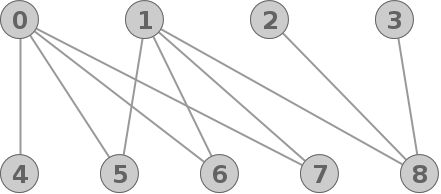
\includegraphics[scale = 0.2]{img/ej3/busqueda_local/k5,4Nocompleto_st0.png} &
			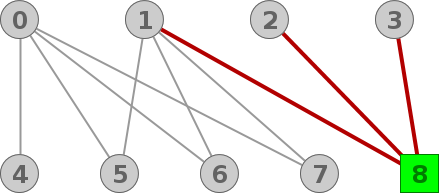
\includegraphics[scale = 0.2]{img/ej3/busqueda_local/k5,4Nocompleto_st1.png} & 
			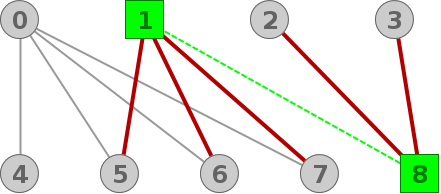
\includegraphics[scale = 0.2]{img/ej3/busqueda_local/k5,4Nocompleto_st2.png} \\
		\hline
		\end{tabular}
	\end{center}
\end{figure}
En este caso el grado promedio es $2,2$ con lo que podr\'ia suceder 
(con las etiquetas correctas) que la busqueda local comience con el
nodo marcado como $8$ en el ejemplo, cosa que en la golosa 
constructiva no pod\'ia suceder.

Para los \'arboles tambi\'en analizaremos el caso extremo presentado 
en la figura \ref{fig:extremo_arboles} y analizaremos nuevamente
la curiosidad de que debido a la relajaci\'on en el criterio de 
selecci\'on del primer nodo en busqueda local, existe una 
construccion alternativa de la clique devuelta por la heur\'istica
aunque sobre este ejemplo la respuesta ser\'a sub-optima.

\begin{figure}[H]
\caption{Resultado sub-\'optimo del ejemplo extremo para \'arboles - 
Forma alternativa}
\begin{center}
		\begin{tabular}{|c||c||c|}
		\hline
		Grafo de entrada & Paso 1 & Paso 2 \\ 
			\hline
			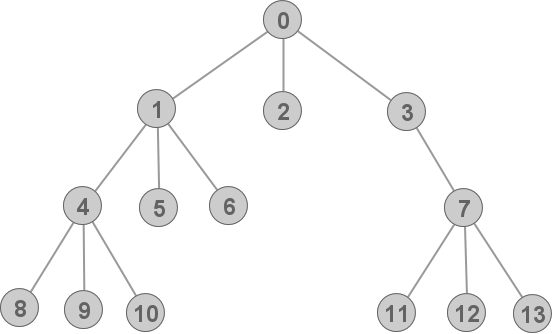
\includegraphics[scale = 0.2]{img/ej3/busqueda_local/extremetree_st0.png} &
			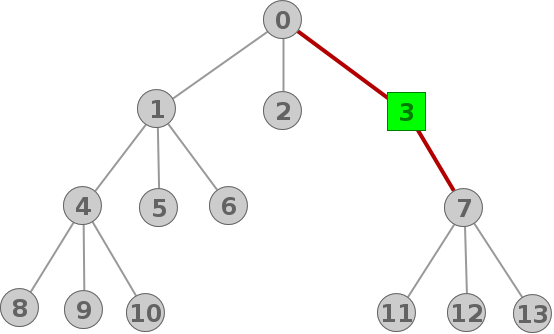
\includegraphics[scale = 0.2]{img/ej3/busqueda_local/extremetree_st11.png} & 
			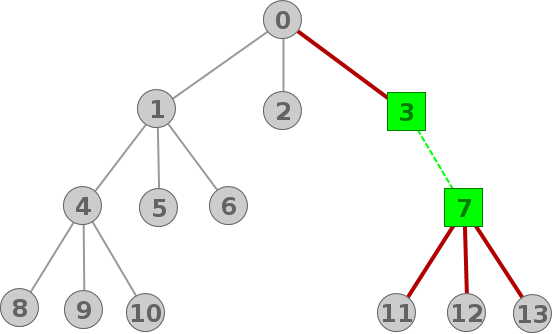
\includegraphics[scale = 0.2]{img/ej3/busqueda_local/extremetree_st12.png} \\
		\hline
		\end{tabular}
	\end{center}
\end{figure}
Notar que aqu\'i el grado promedio es aproximadamente $1,8$ con lo que 
el nodo identificado como $3$ en el ejemplo es elegible como
primer nodo de $K$ pues $2 > 1,8$.

\subsubsection{Estrella + Puente + CMF}

En esta familia, siguiendo con la idea de las \'ultimas dos analizadas
podemos ver que que para llegar a la soluci\'on \'optima hay muchos 
m\'as puntos de inicio que en la golosa constructiva. Por ejemplo
el primer nodo puede estar en $K_{\Delta -1}$ y no ser siquiera $v'$ 
(ver Figura \ref{fig:epcmf_carac}), en los casos en los que esto 
suceda, en la variante b\'asica, la busqueda local elegir\'a
$\left\lfloor \frac{\Delta -1}{2} \right\rfloor$ nodos de $K_{\Delta -1}$. 
Si estos nodos incluyen a $v'$, termina pues no quedan candidatos que
hagan crecer la soluci\'on parcial, si no lo incluyen hay dos posibilidades:

\begin{itemize}
	\item $\Delta$ par: La cantidad de nodos en $K_{\Delta -1}$ ser\'a impar 
	y entonces la soluci\'on crece hasta alcanzar
	$\left\lfloor \frac{\Delta -1}{2} \right\rfloor$ nodos que por hip\'otesis
	no incluyen a $v'$, en el siguiente paso el \'unico candidato restante
	que hace crecer la soluci\'on en una arista es $v'$ y por ello lo agrega 
	a la soluci\'on, terminando con una soluci\'on \'optima.
	Ejemplo (con $v = 0$, $v' = 7$):
	\begin{center}
	\begin{tabular}{|c||c|}
		\hline
		Grafo entrada & 
		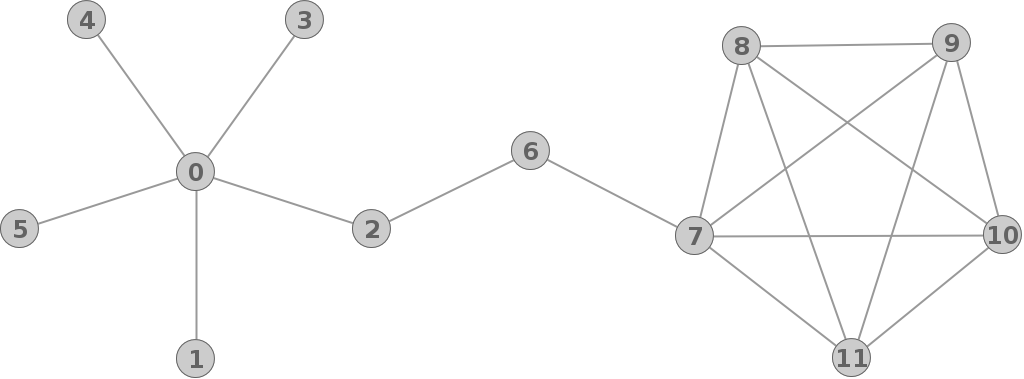
\includegraphics[scale = 0.2]{img/ej3/busqueda_local/estrellaPuenteCMFImpar.png} \\
		\hline
		Primer paso &
		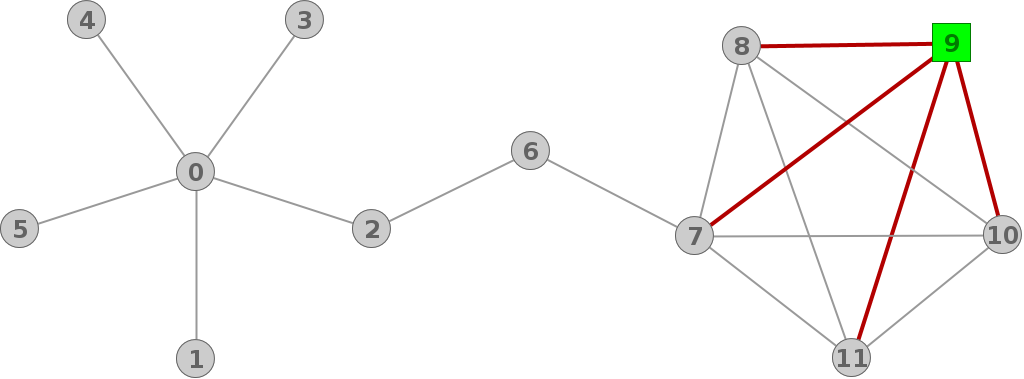
\includegraphics[scale = 0.2]{img/ej3/busqueda_local/estrellaPuenteCMFImpar_st01.png} \\
		\hline
		Segundo paso &
		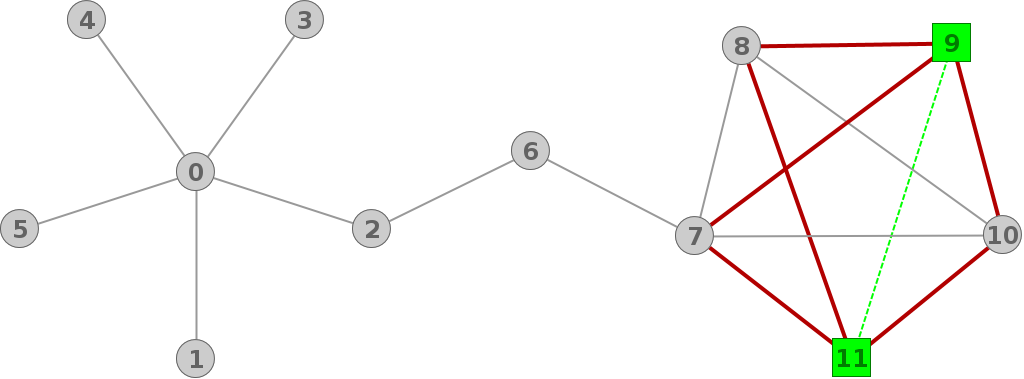
\includegraphics[scale = 0.2]{img/ej3/busqueda_local/estrellaPuenteCMFImpar_st02.png} \\
		\hline
		Tercer paso &
		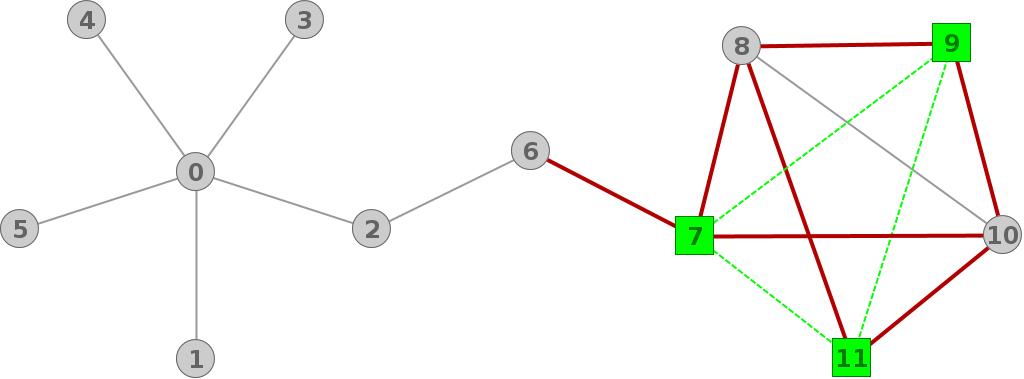
\includegraphics[scale = 0.2]{img/ej3/busqueda_local/estrellaPuenteCMFImpar_st03.png} \\
		\hline

	\end{tabular}
	\end{center}


	\item $\Delta$ impar: La cantidad de nodos en $K_{\Delta -1}$ ser\'a par, 
	en este caso la soluci\'on crece hasta alcanzar $\frac{\Delta -1}{2}$ nodos
	que no incluyen a $v'$, llegados a este punto la soluci\'on no puede crecer
	para incluir a $v'$ ya que de hacerlo la frontera de la soluci\'on ser\'ia
	la misma que en el paso anterior y el algoritmo no se comporta de esta manera.
	Por ende la soluci\'on devuelta es sub-\'optima.
	Ejemplo (con $v = 0$, $v' = 13$):
	\begin{center}
	\begin{tabular}{|c||c|}
		\hline
		Grafo entrada & 
		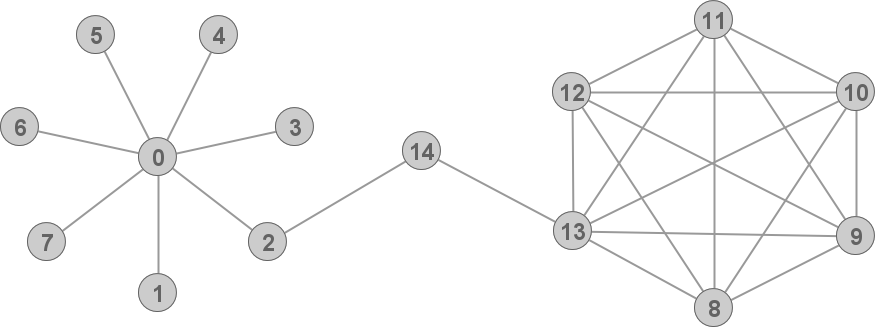
\includegraphics[scale = 0.2]{img/ej3/busqueda_local/estrellaPuenteCMFPar.png} \\
		\hline
		Primer paso &
		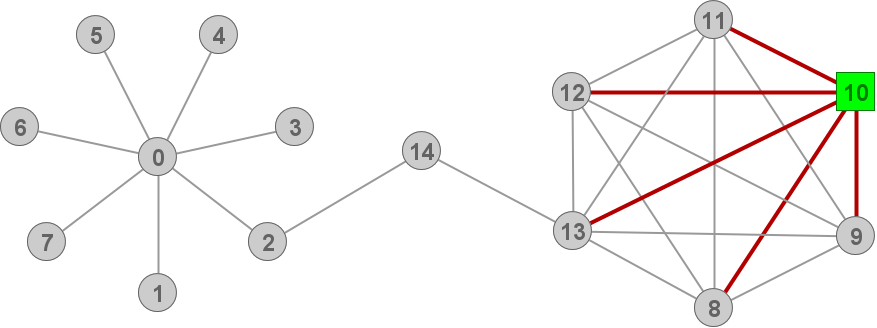
\includegraphics[scale = 0.2]{img/ej3/busqueda_local/estrellaPuenteCMFPar_st01.png} \\
		\hline
		Segundo paso &
		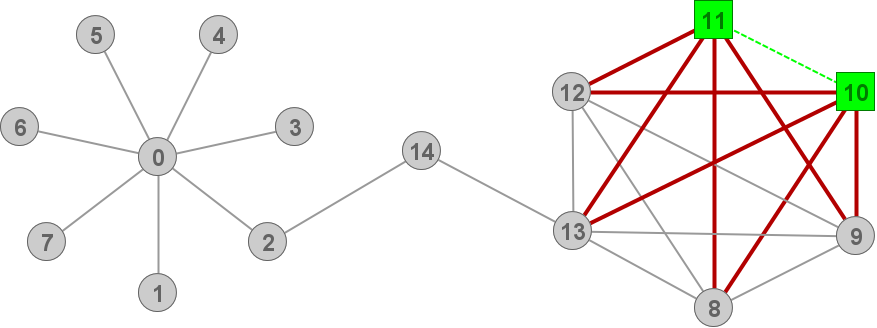
\includegraphics[scale = 0.2]{img/ej3/busqueda_local/estrellaPuenteCMFPar_st02.png} \\
		\hline
		Tercer paso &
		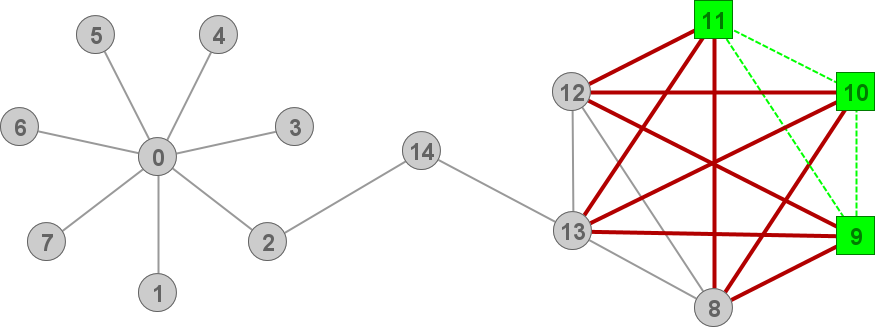
\includegraphics[scale = 0.2]{img/ej3/busqueda_local/estrellaPuenteCMFPar_st03.png} \\
		\hline

	\end{tabular}
	\end{center}


\end{itemize}

Notar que en la variante \emph{Mejor Vecino} evita el resultado sub-\'optimo en 
el \'ultimo caso (bajo las hip\'otesis del mismo), esto tambi\'en se logra con
la variante \emph{Vecindad Con Intercambio}.

Hay otros posibles comportamientos de la heur\'istica sobre la misma familia de
grafos, que el algoritmo comience la soluci\'on en uno de los nodos del puente o
que la comience en el centro de la estrella.

Que comience la soluci\'on sobre el puente es un caso que t\'ipicamente no va a 
suceder, si es un puente simple (camino simple) la \'unica forma de que sucediera
ser\'ia si el puente es lo suficientemente largo para bajar el grado promedio a
un valor menor a dos, si el puente no es un camino simple y en cambio tiene nodos
extra, el puente no tendr\'a que ser tan largo pero siempre se deber\'a cumplir
que el nodo inicial de la soluci\'on tenga grado mayor al grado promedio del grafo.

Cuando la soluci\'on se inicia en el centro de la estrella, la busqueda local 
se estanca en el m\'aximo local debido al puente que une la estrella con $K_{\Delta -1}$,
de hecho, esta familia fue dise\~nada con el objetivo de asegurar precisamente
este estancamiento.
		
\subsubsection{Estrella + CMF}

Para esta familia, nuevamente se tiene que cuando el el orden en el que el algoritmo
construye la soluci\'on no coincide con el orden que utiliza la golosa constructiva, 
la heur\'istica puede llegar a construir el resultado \'optimo.
Supongamos que la busqueda local comienza por un nodo perteneciente a $K_{\Delta -1}$
(ver figura \ref{fig:ecmf_carac}). El an\'alisis es completamente an\'alogo al
realizado para la familia anterior bajo las mismas condiciones. La excepci\'on
se da cuando comienza por $v$, ya que puede devolver o bien la misma soluci\'on que
la golosa constructiva o bien una soluci\'on \'optima (esto en su versi\'on standard, 
en la versi\'on de \emph{Mejor Vecino} devuelve el mismo resultado de la golosa).

El caso notable para esta familia es cuando la soluci\'on empieza por $v'$, puesto 
que la heur\'istica se estanca en el \'optimo local y no puede salir del mismo, ni siquiera
en su variante \emph{Vecindad Con Intercambio}. Veamos c\'omo sucede esto: el 
algoritmo comienza (por nuestra hip\'otesis) en el nodo $v'$, en el siguiente paso
la vecindad esta dada por la clique de nodos $v, v'$ cuya frontera (llamemosle 
$\delta(SBL)$) es mayor a la calculada en el paso anterior. Tenemos entonces
\[ d(v') = \Delta -1 \]
\[ d(v) = \Delta \]
\[ \delta(SBL) = (\Delta -1) -1 + \Delta -1 = 2 \Delta -3 \]
Ejemplo (con $v=3$ y $v'=8$):
\begin{center}
	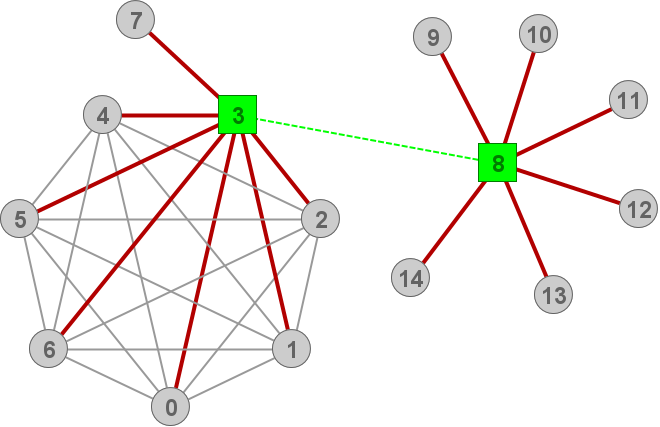
\includegraphics[scale = 0.3]{img/ej3/busqueda_local/estrellaCMF_st02.png} \\
\end{center}

Queda claro que no puede agregar nodos por la naturaleza de la familia, 
tampoco podr\'a reducir nodos ya que la frontera disminuir\'ia. La \'unica
alternativa ser\'ia intercambiar nodos, con la idea de abandonar $v'$ y 
reemplazarlo por alg\'un nodo de $K_{\Delta -1}$, llamesmole $x$. 
Supongamos por un momento, 
y solo a modo de an\'alisis que esto fuera posible, llamemos a la frontera
de esta hipot\'etica soluci\'on parcial $\delta(SBL')$, tendr\'iamos

\[ d(v) = \Delta \]
\[ d(x) = \Delta -2 \]
\[ \delta(SBL') = \Delta -1 + (\Delta -2) -1 = 2 \Delta -4 \]
Ejemplo (con $v=3$ y $x=2$):
\begin{center}
	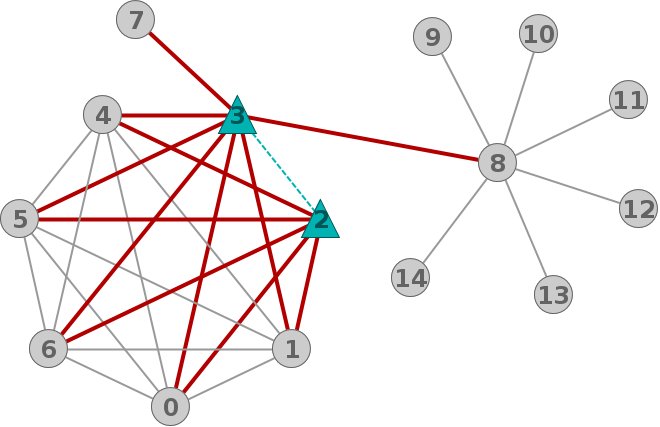
\includegraphics[scale = 0.3]{img/ej3/busqueda_local/estrellaCMF_st12.png} \\
\end{center}

Luego $\delta(SBL') < \delta(SBL)$ y entonces el cambio nodo a nodo no 
mejorar\'ia la funci\'on objetivo, con lo cual el algoritmo jamas efectua
el cambio y la soluci\'on no puede escapar a este estancamiento local.

La soluci\'on \'optima tendr\'ia la siguiente forma:
\begin{center}
	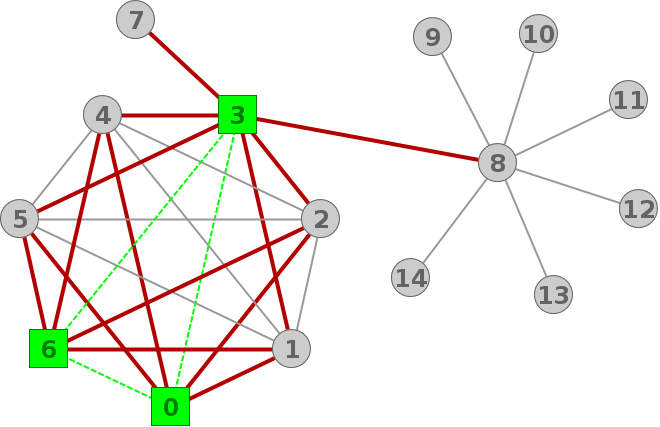
\includegraphics[scale = 0.3]{img/ej3/busqueda_local/estrellaCMF_st22.png} \\
\end{center}
